\chapter{SM}
Dette afsnit beskriver designet af styringsmodulet, SM.
\section{Klassens ansvar}
Styringsmodulet har til ansvar at holde styr på levelsensoren og værdierne fra VBTE. Den kommunikere med KI og VBTE med indbyggede API'er fra Cypress PSoC 5 biblioteker. 
\section{Klassediagram}
Nedenfor ses klassediagrammet for SM. Bemærk at koden dog er i C men for overblikket er der lavet klassediagram.
\begin{figure}[H]
\centering
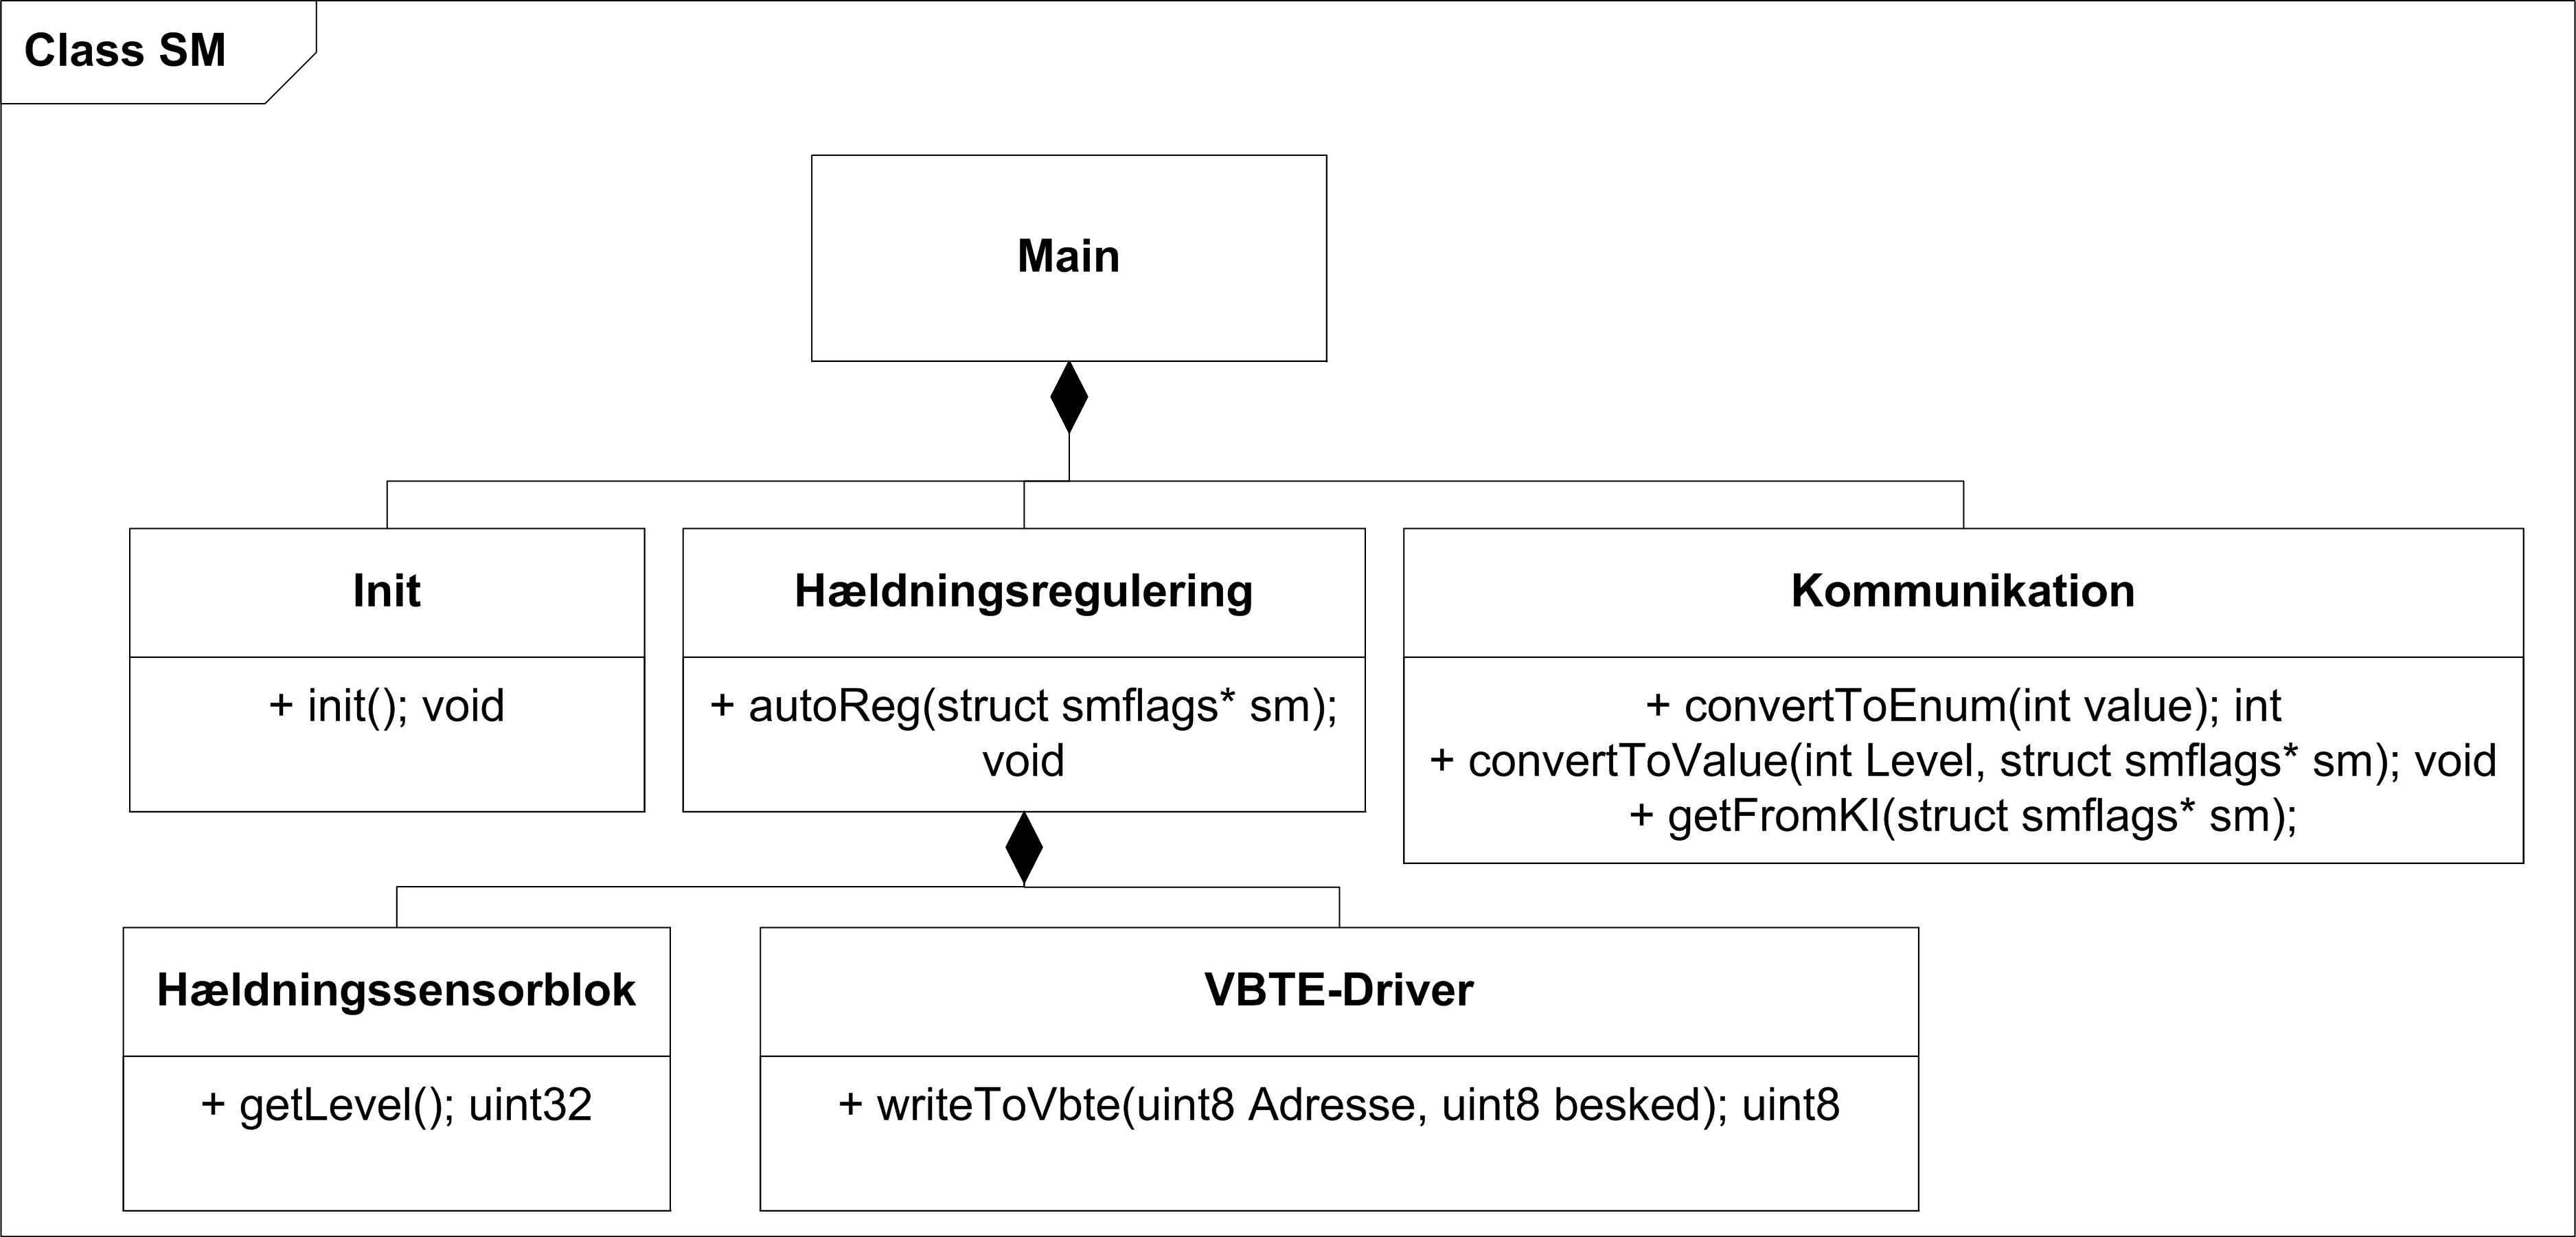
\includegraphics[width=1\textwidth]{billeder/smKlassediagram}
\caption{På figuren ses klassediagrammet for SM}
\end{figure}
\section{Funktioner}
bla bla
\section{Variabler}
\begin{table}[H]
\begin{tabular}{|l|p{10cm}|}
\hline
\cellcolor[gray]{0.8}\textbf{Variabel} &\cellcolor[gray]{0.8} \textbf{Beskrivelse}\\ \hline
\texttt{autoflag} & Denne variable er et flag der holder styr på automatisk regulering .\\ \hline
\texttt{manuflag} & Et flag til at holde styr på manuel regulering.\\ \hline
\texttt{levelVal} & En variable med vores level værdi.\\ \hline
\texttt{VBTE1Niveau og VBTE2Niveau} & Holder styr på vandniveauet i ballasttanke i \%. \\ \hline
\texttt{VBTE1Status og VBTE2Status} & Holder styr op tilgængelighed for VBTE1 og 2.\\ \hline
\texttt{vinkelVal} & Indeholder værdien for manuel regulering.\\ \hline
\end{tabular}
\end{table}
Alle variabler er indkapslet i en struct navngivet "smflags".
\section{Funktionsbeskrivelser}
\subsection{Init}
\subsubsection{Ansvar}
Denne header har til ansvar at sørge for alle komponenter opretter og initieret.
\texttt{\textcolor{blue}{void} init( \textcolor{blue}{void});} 
\begin{table}[H]
\begin{tabular}{l p{12.5cm}}
\hline
Beskrivelse:& Funktionen anvender API'et fra Cypress componenter og står for at initiere og starte vores PSoC hardware. Den sætter også et register tilhørende vores Accelerometer. \\
Parametre:&ingen\\
Returværdi:&ingen\\
\end{tabular}
\end{table}
% spacer %
\subsection{Levelsensor}
\subsubsection{Ansvar}
Denne header har til ansvar at hente levelværdien ind fra vores accelerometer.
\texttt{\textcolor{blue}{uint32} getLevel( \textcolor{blue}{void});} 
\begin{table}[H]
\begin{tabular}{l p{12.5cm}}
\hline
Beskrivelse:& Funktionen anvender API'et fra Cypress componenter og venter på at vores ADC henter convertere det analoge signal. Funktionskald for ADC ses i PSoC databladet. \\
Parametre:&ingen\\
Returværdi:&\texttt{\textcolor{blue}{uint32} levelVal}\\
\end{tabular}
\end{table}
% spacer %
\subsection{autoReg}
\subsubsection{Ansvar}
Denne header har til ansvar at styre automatisk regulering.
\texttt{\textcolor{blue}{void} autoReg( \textcolor{blue}{struct} smflags* sm);} 
\begin{table}[H]
\begin{tabular}{l p{12.5cm}}
\hline
Beskrivelse:& autoReg anvender værdier fra VBTE moduler samt KI til at holde systemet i et bestemt level. Funktionen starter med at checke på automatisk og manuel styrings flagene. Derefter kalder den getLevel agere ud fra niveauet. Funktionen vil altid tømme fra en tank før den begynder at fylde en anden.\\
Parametre:&\texttt{\textcolor{blue}{struct} smflags* sm}\\
Returværdi:&ingen\\
\end{tabular}
\end{table}
% spacer %
\subsection{I2C\_Kom}
\subsubsection{Ansvar}
Denne header har til ansvar at kommunikere med VBTE modulerne.
\texttt{\textcolor{blue}{uint8} writeToVbte( \textcolor{blue}{uint8} Adresse, \textcolor{blue}{uint8} besked);} 
\begin{table}[H]
\begin{tabular}{l p{12.5cm}}
\hline
Beskrivelse:& writeToVbte anvender I2C fra Cypress PSoC 5 API til at skrive til VBTE modulerne. Den tager adressen og beskeden man skal sende og sender til pågældende enhed. Derefter venter den på svar som den så returnere. \\
Parametre:&\texttt{\textcolor{blue}{uint8} Adresse}\\
 &\texttt{\textcolor{blue}{uint8} besked}\\
Returværdi:&\texttt{\textcolor{blue}{uint8} VbteNiveau}\\
\end{tabular}
\end{table}
% spacer %
\subsection{KI\_KOM}
\subsubsection{Ansvar}
Denne header har til ansvar at kommunikere med KI enheden.\\
\texttt{\textcolor{blue}{int} convertToEnum( \textcolor{blue}{int} value);} 
\begin{table}[H]
\begin{tabular}{l p{12.5cm}}
\hline
Beskrivelse:& funktionen tager en level værdi ind for så at konvertere den til en Enum(integer) som den returnere.\\
Parametre:&\texttt{\textcolor{blue}{int} value}\\
Returværdi:&\texttt{\textcolor{blue}{int} Enum}\\
\end{tabular}
\end{table}
\texttt{\textcolor{blue}{void} convertToValue(\textcolor{blue}{int} Level,   \textcolor{blue}{struct} smflags* sm);} 
\begin{table}[H]
\begin{tabular}{l p{12.5cm}}
\hline
Beskrivelse:& Funktionen tager en enum og en pointer som den så konvertere til en level værdi og sætter i sm structen.\\
Parametre:&\texttt{\textcolor{blue}{int} Level},\\
 &\texttt{\textcolor{blue}{struct} smflags* sm}\\
Returværdi:&ingen\\
\end{tabular}
\end{table}
\texttt{\textcolor{blue}{void} getFromKI( \textcolor{blue}{struct} smflags* sm);} 
\begin{table}[H]
\begin{tabular}{l p{12.5cm}}
\hline
Beskrivelse:& Funktionen anvender UART fra Cypress PSoC 5 API'en til at modtage en besked fra KI modulet som den så vurdere og agere på. Når den har modtaget noget sender den en ack tilbage til KI modulet. Derefter handler den og hvis det er nødvendigt sender data til KI. \\
Parametre:&\texttt{\textcolor{blue}{struct} smflags* sm}\\
Returværdi:&ingen\\
\end{tabular}
\end{table}
% spacer %
\section{Eventuelle Sekvensdiagrammer og state machines}
Måske kommer de senere?